\documentclass[10pt,a4paper]{article}
\usepackage[margin=2.2cm]{geometry}
\usepackage{fontspec}
\usepackage{amsmath,amssymb}
\usepackage{booktabs,graphicx,float,xcolor,array}
\usepackage[font=small,labelfont=bf]{caption}
\usepackage{enumitem}
\usepackage[colorlinks=true,linkcolor=blue!50!black,urlcolor=blue!50!black,citecolor=blue!50!black]{hyperref}
\setlist{itemsep=2pt,topsep=3pt}
\graphicspath{{../figures/}{../figures/explained/}}
\newcommand{\tabin}[1]{\input{tables/#1.tex}}
\newcommand{\code}[1]{\texttt{#1}}

\title{\textbf{Scaling Neural Bayesian Networks with graph size and graph complexity}\\[4pt]
\large What was changed in NBN, why the answers stay the same, and what it buys}
\author{Alfredo (\code{alfredo\_claude}) for Giovanni Briglia}
\date{17 October 2026 --- branch \code{feat/scaling-study} (from \code{master} @ \code{61831fa}), local, not pushed}

\begin{document}
\maketitle

\section*{Summary}

\textbf{Question.} Can NBN scale with the number of nodes and with the number of edges of the
graph, under a tight compute budget, without changing what it computes? Discrete networks are
compared with pgmpy (maximum-likelihood fitting and variable elimination), continuous
non-Gaussian networks with Pyro.

\textbf{Answer.} \emph{Yes for graph size; partly for graph complexity.} The part that does
not scale is a theorem, not an implementation detail. Under 1 CPU thread, 4\,GB and 30\,s per
run, after the changes on this branch:
\begin{itemize}
  \item Fitting, sampling queries, S4 sets and non-Gaussian queries reach the largest size
  tested (5\,000 nodes). Exact queries also reach it when the graph stays ``thin'' (bounded
  tree-width): 0.17\,s for 10 queries, 8$\times$ faster than pgmpy.
  \item Exact queries on dense graphs stop at about 100 nodes for \emph{every} library (NBN,
  NBN before, pgmpy). The cost is exponential in the tree-width, and finding the best order is
  NP-hard. For these graphs the branch adds \emph{certified} sampling answers: intervals that
  contain the true value with probability $\geq 95\%$. All 528 checked intervals did, and they
  reach 5\,000 nodes at 1.5\,s per query.
  \item The changes are 3.4--51$\times$ faster on the same answers, with 8$\times$ less memory
  for tables with many parents. The biggest gains come from removing bookkeeping, not from
  faster arithmetic.
  \item Two real limits remain: rare evidence (any sampler needs $\sim 1/P(e)$ samples), and
  tables with many parents (fast to fit now, but statistically poor because of data
  fragmentation).
\end{itemize}

\begin{figure}[H]\centering
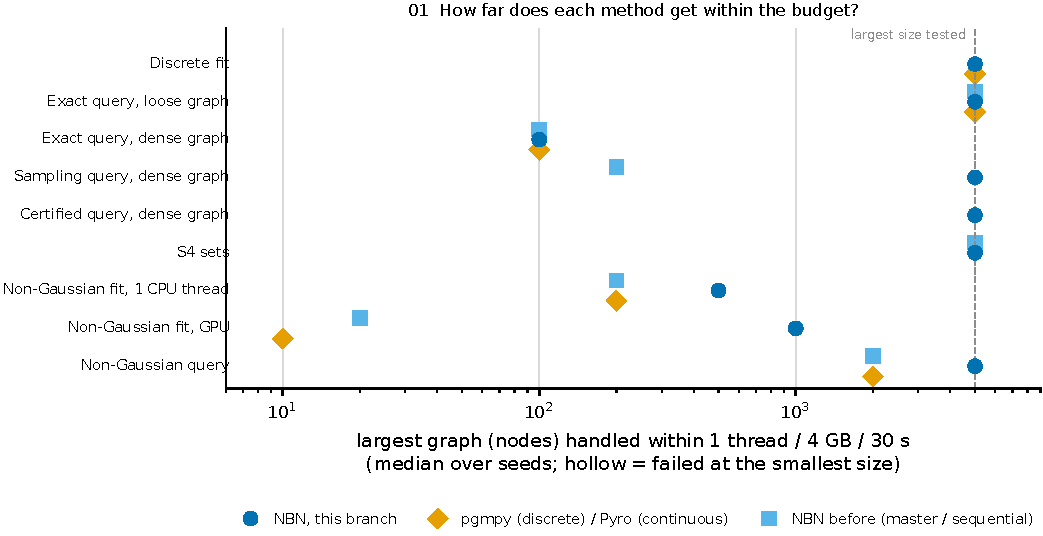
\includegraphics[width=0.93\linewidth]{01_overview_frontier.pdf}
\caption{Largest graph each method handles within the budget (median over seeds; 5\,000 =
largest size tested). Dark circles: this branch; light squares: NBN before (master, or the old
one-node-at-a-time training); diamonds: pgmpy (discrete) or Pyro (continuous).}
\label{fig:overview}
\end{figure}
\tabin{q1}

\section{Set-up}

\paragraph{Budget.} Every measurement runs in a fresh process with \textbf{1 CPU thread} (torch
and BLAS pinned), an \textbf{RSS watchdog at 4\,GB} (killed $\to$ ``oom'') and \textbf{30\,s}
for the timed region ($\to$ ``timeout''). Imports and data loading are not charged. Separate
arms run the same cells on the Apple M5 GPU (MPS) and on the whole CPU (10 threads, 24\,GB).
Exact inference in NBN is told the budget (75\% of the cap), so it refuses a query it cannot fit
instead of being killed.

\paragraph{Graphs.} Random DAGs in a fixed topological order:
\begin{center}\small\resizebox{\linewidth}{!}{\begin{tabular}{lll}\toprule
family & parents of node $j$ & what it stresses \\ \midrule
dense (Erdős--Rényi) & $\min(j, 8, \mathrm{Poisson}(d))$ among \emph{all} earlier nodes & size and complexity: tree-width grows with $n$\\
loose (window 5) & same count, among the 5 previous nodes & size only: tree-width $\leq 5$ at any $n$\\
fixed in-degree & exactly $\min(j, d)$ earlier nodes & table size $K^{d+1}$\\ \bottomrule
\end{tabular}}\end{center}
x-axes: nodes $n\in\{10,\dots,5000\}$ at mean in-degree 2; edges (mean in-degree 1 to 8 at fixed
$n$); in-degree 2 to 20 (30 nodes).

\paragraph{Data.} Discrete: $K=3$ values, random CPT logits $\mathcal N(0,1)$. For the
in-degree sweep the CPTs are additive in logit space, so the ground truth stays compact.
Continuous non-Gaussian: every node is a 3-component Gaussian mixture whose means are linear in
the standardised parents, with skewed offsets. 95\% of nodes reject normality; the median excess
kurtosis is 1.3. Each problem has 10\,000 training rows and 2\,000 test rows. Discrete queries
are $P(Y \mid 5 \text{ observed nodes})$; continuous queries are
$P(Y>\mathrm{median}\mid 3 \text{ observed nodes in } Y\text{'s Markov blanket})$; 10 queries
per graph, 3 seeds for discrete queries.

\paragraph{Methods.}
\begin{center}\small\resizebox{\linewidth}{!}{\begin{tabular}{lll}\toprule
task & NBN & baseline \\ \midrule
discrete fit & count MLE (dense or sparse table) & pgmpy \code{MaximumLikelihoodEstimator} \\
discrete query & exact VE; LW (100k samples); certified LW (200k, $\delta=0.05$) & pgmpy \code{VariableElimination} (default order) \\
S4 sets & KL intervals per node / batched; L1 balls & --- \\
non-Gaussian fit & mixture density network (MDN), sequential vs \textbf{stacked} & Pyro SVI, same model, same Adam steps \\
non-Gaussian query & LW, 10k samples & Pyro importance sampling (vectorised; and \code{Importance}) \\ \bottomrule
\end{tabular}}\end{center}

\section{What was changed}

Each change keeps the same estimator, or the same answer: exactly for exact methods, and in
distribution for samplers. Each has tests. The full unit and integration suites pass, and ruff
and mypy are clean.

\begin{table}[H]\centering\small
\caption{Changes on the branch (14 commits).}\label{tab:changes}
\resizebox{\linewidth}{!}{%
\begin{tabular}{p{0.27\linewidth}>{\raggedright\arraybackslash}p{0.25\linewidth}p{0.42\linewidth}}\toprule
change & where & why the answers do not change \\ \midrule
Incremental greedy min-fill & \code{\_elimination\_order.py} & re-scores only the 2-neighbourhood of the eliminated node; identical order to the old loop (500 random graphs) \\
Evidence conditioned out of the ordering graph; cheaper of new and old order kept & same & an order changes cost, never the answer; never costlier by VE factor sizes \\
Incremental \code{DAG.induced\_width} & \code{dag.py} & same value, same tie-breaking (300 random graphs) \\
Barren-node pruning in likelihood weighting (LW) & \code{likelihood\_weighting.py} & nodes outside the ancestors of target $\cup$ evidence cannot change the weights or the target (K\&F Ex.\ 3.8) \\
Inverse-CDF categorical sampling & \code{categorical\_table.py} & exactly the categorical law of the CPT row; zero-probability classes never drawn \\
LW particles in passes & \code{likelihood\_weighting.py} & particles are i.i.d.; memory $O(\text{pass}\times n)$ \\
Stacked fitting \code{fit(method="stacked")} + closed-form mixture-NLL backward & \code{stacked.py}, \code{fit.py} & per-node objective, Adam (element-wise) and per-node clipping unchanged; equal to sequential fitting to $2\cdot 10^{-6}$ with full batches; backward equal to autograd to $10^{-14}$ \\
Sparse table mechanism & \code{SparseCategorical-} \code{TableMechanism} & the dense MLE table is uniform on rows without data; identical log-probabilities, tables and sampling law \\
Batched \code{interval\_sets} & \code{builders.py} & bit-identical to per-node \code{interval\_set} \\
\code{certified\_query} & \code{certified.py} & new answer type (bounds with a declared level), not a new model; see Appendix B \\
Width bounds; opt-in query-width routing & \code{tensor\_ve.py}, \code{hybrid.py} & diagnostics; routing is opt-in (default unchanged) \\ \bottomrule
\end{tabular}}
\end{table}

\section{What each change buys}

\begin{figure}[H]\centering
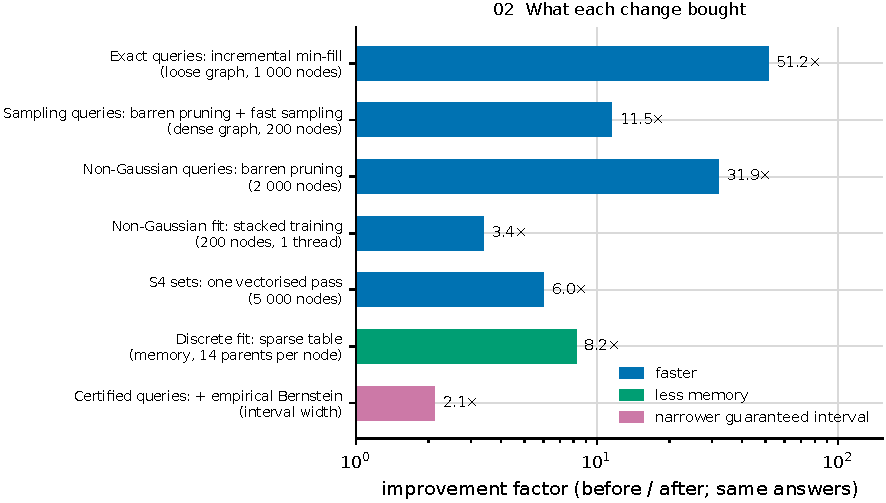
\includegraphics[width=0.8\linewidth]{02_what_each_change_bought.pdf}
\caption{Before/after factor of each change, at a representative size.}\label{fig:bought}
\end{figure}
\tabin{q2}

\paragraph{Exact queries were slow because of bookkeeping.} Before, 95\% of the exact-query time
was spent choosing the elimination order. The old loop re-scored every node and copied the whole
graph at every step. The incremental version returns the same order; total time drops 13--15$\times$
(Table~\ref{tab:q3}).
\begin{figure}[H]\centering
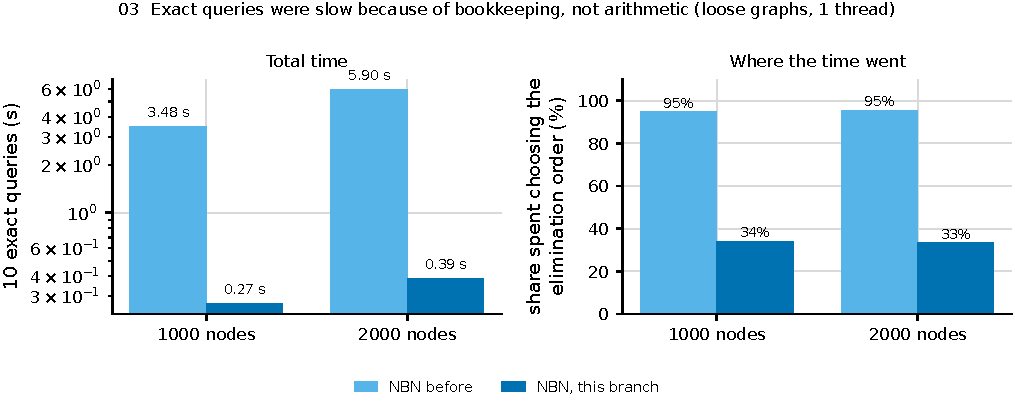
\includegraphics[width=0.9\linewidth]{03_where_exact_query_time_went.pdf}
\caption{Ten exact queries on loose graphs, before and after.}\label{fig:ordering}
\end{figure}
\tabin{q3}

\paragraph{Sampling only what can affect the answer.} A sampling query needs only the ancestors
of its target and its evidence. On a 5\,000-node dense graph that is 5\% of the nodes (3\% in
the non-Gaussian case). Before, every query sampled every node.
\begin{figure}[H]\centering
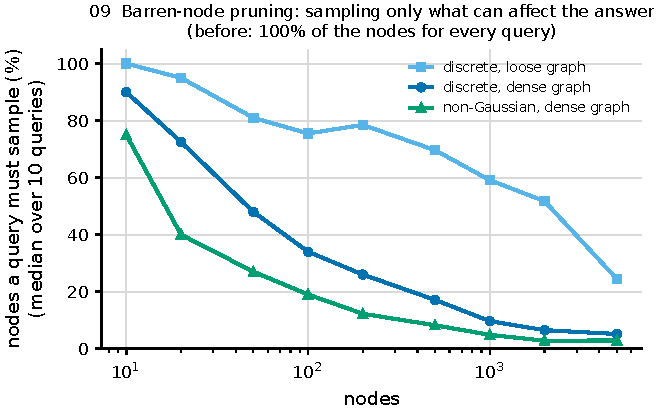
\includegraphics[width=0.62\linewidth]{09_barren_pruning.pdf}
\caption{Share of nodes a sampling query must touch (median of 10 queries).}\label{fig:pruning}
\end{figure}
\tabin{q9}

\paragraph{Stacked fitting.} The likelihood splits into one term per node, and each node's
best fit can be found independently (K\&F Prop.\ 17.1, p.\ 725). The old path trained one node
at a time, paying a fixed overhead per node. Stacking trains all nodes of one architecture as
one batched network: about 30\,ms per node on one CPU thread, against 95\,ms sequential and
130\,ms for Pyro. On the GPU it is 15\,ms per node, where sequential training costs 800\,ms or
more per node. Fit quality is the same.
\begin{figure}[H]\centering
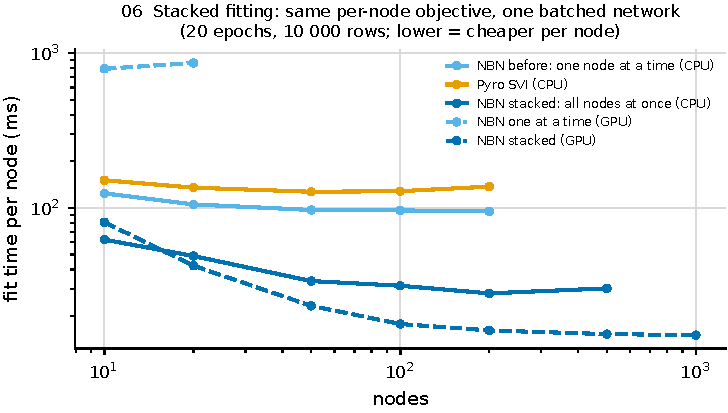
\includegraphics[width=0.65\linewidth]{06_stacked_fit_cost_per_node.pdf}
\caption{Non-Gaussian fit time per node.}\label{fig:stacked}
\end{figure}
\tabin{q6}

\paragraph{Sparse tables.} A full table needs $K^{p+1}$ numbers for $p$ parents. With $N$ rows,
at most $N$ parent combinations are ever seen, and the MLE is uniform on all others.
\begin{figure}[H]\centering
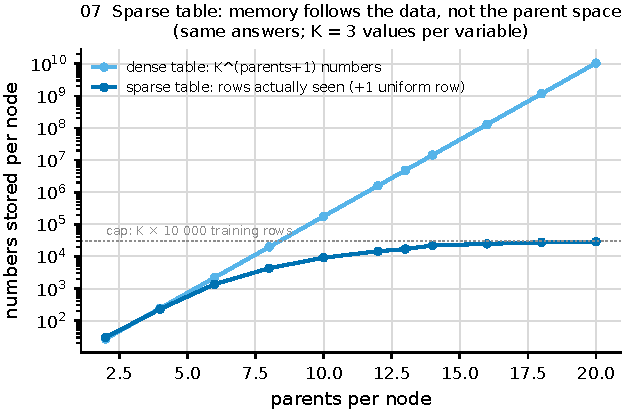
\includegraphics[width=0.6\linewidth]{07_sparse_table_memory.pdf}
\caption{Numbers stored per node, dense vs sparse table.}\label{fig:sparse}
\end{figure}
\tabin{q7}

\section{Results by task}

\subsection{Discrete fitting (vs pgmpy)}
NBN and pgmpy give identical tables on every problem: same total-variation error to the truth,
same checksum. With nodes, NBN takes 1.48\,s at 5\,000 nodes against 3.95\,s for pgmpy. With
edges, pgmpy grows 8$\times$ (0.12$\to$0.92\,s) while NBN stays near 0.1\,s.
\begin{figure}[H]\centering
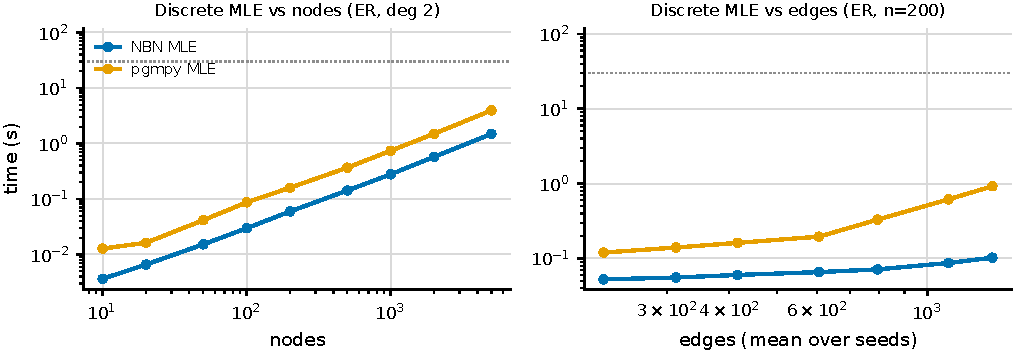
\includegraphics[width=0.85\linewidth]{discrete_fit.pdf}
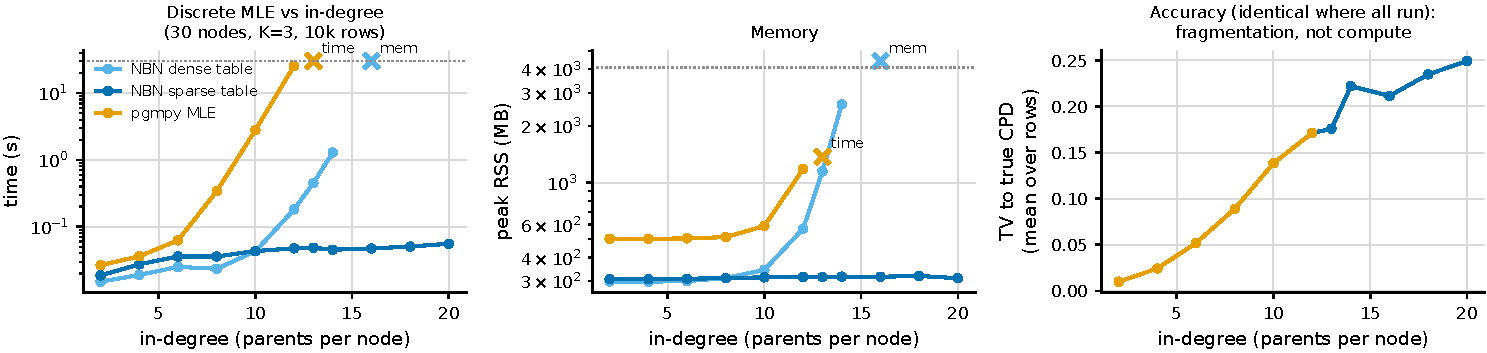
\includegraphics[width=\linewidth]{discrete_fit_indeg.pdf}
\caption{Discrete fit vs nodes and edges (top), and vs parents per node (bottom).}\label{fig:dfit}
\end{figure}
\paragraph{Many parents: a statistical limit.} Computing is solved; statistics is not. With 20
parents almost every parent combination is seen once, and the fitted table's error grows
25$\times$. The sample size needed grows exponentially in the in-degree (K\&F Cor.\ 17.3,
p.\ 775). Past about 10 parents a different model type is needed, which is a modelling choice
and was not made here.
\begin{figure}[H]\centering
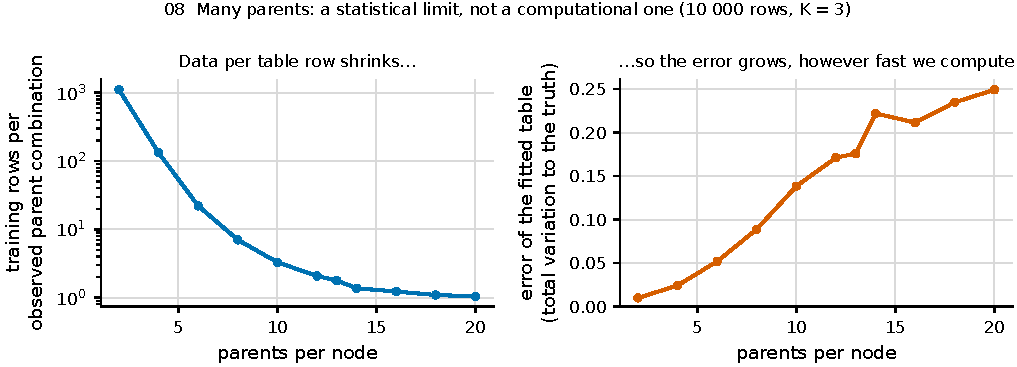
\includegraphics[width=0.9\linewidth]{08_data_fragmentation.pdf}
\caption{Data per table row and error of the fitted table.}\label{fig:frag}
\end{figure}
\tabin{q8}

\subsection{Discrete queries (vs pgmpy)}
NBN and pgmpy exact answers agree to $1.9\cdot10^{-7}$ on 450 queries. On loose graphs exact
inference scales to 5\,000 nodes. On dense graphs every exact method stops early: pgmpy runs
out of memory at 200 nodes. Within the budget NBN answers 90\% of queries exactly at 200 nodes,
47\% at 500 and $\sim$25\% at 2\,000--5\,000, and refuses the rest instead of crashing. With the
whole machine (10 threads, 18\,GB) the exact share stays about the same, because more memory
buys little against exponential growth.
\begin{figure}[H]\centering
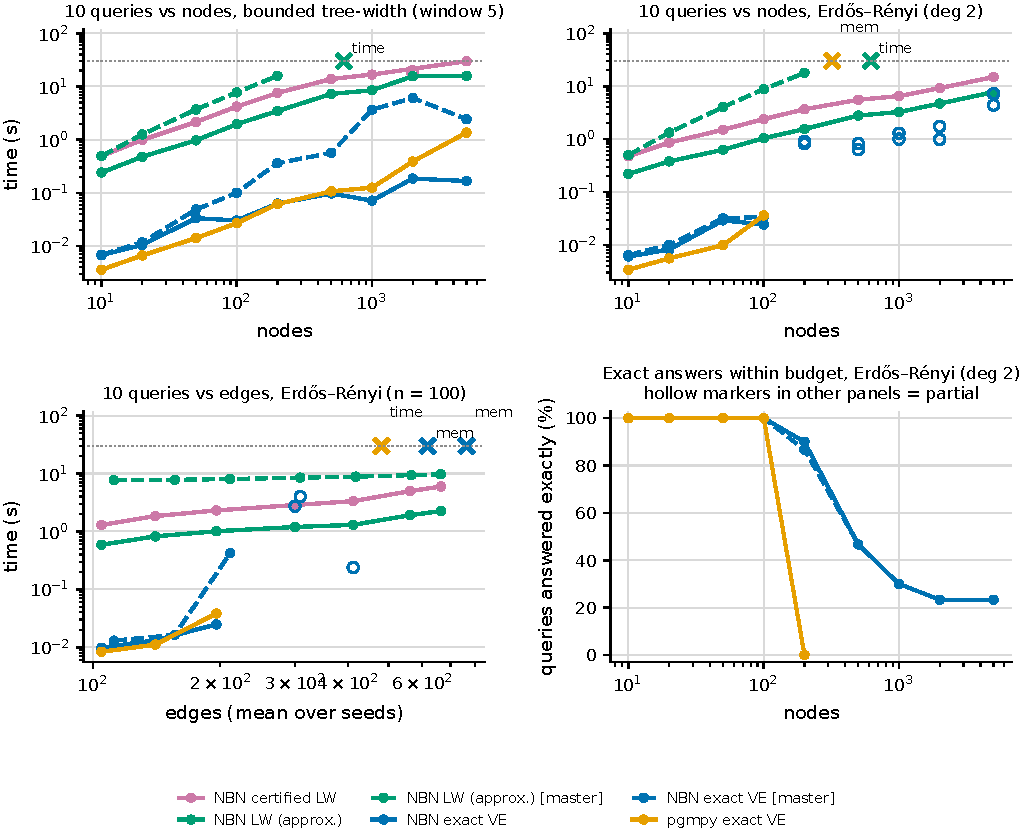
\includegraphics[width=\linewidth]{discrete_infer.pdf}
\caption{Discrete queries: time for 10 queries vs nodes and edges, and the share of exact
answers on dense graphs. Hollow markers: some queries or seeds failed.}\label{fig:dinfer}
\end{figure}

\paragraph{The tree-width wall.} The biggest table in an exact computation has $K^{w+1}$ entries,
where $w$ is the query's induced width. Variable-elimination cost is exponential in $w$ (K\&F
Thm 9.6, p.\ 309); the best order is NP-hard to find (Thm 9.7, p.\ 310); even approximate
inference with evidence is NP-hard in the worst case (Thm 9.4, p.\ 291).
\begin{figure}[H]\centering
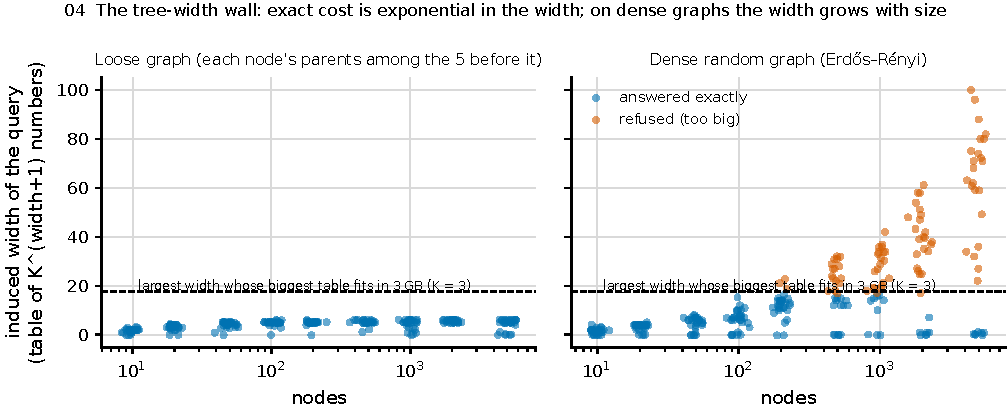
\includegraphics[width=\linewidth]{04_treewidth_wall.pdf}
\caption{Induced width of each query vs graph size.}\label{fig:wall}
\end{figure}
\tabin{q4local}
\tabin{q4er}

\subsection{Certified sampling answers}
For dense graphs, where exact answers are out of reach, \code{certified\_query} returns, for every
class $y$, an interval $[\ell_y, u_y]$. With probability $\geq 1-\delta$ all the intervals hold
together (Appendix B). Plain likelihood weighting gives only a point estimate and an effective
sample size, which is a heuristic (K\&F p.\ 504).
\begin{figure}[H]\centering
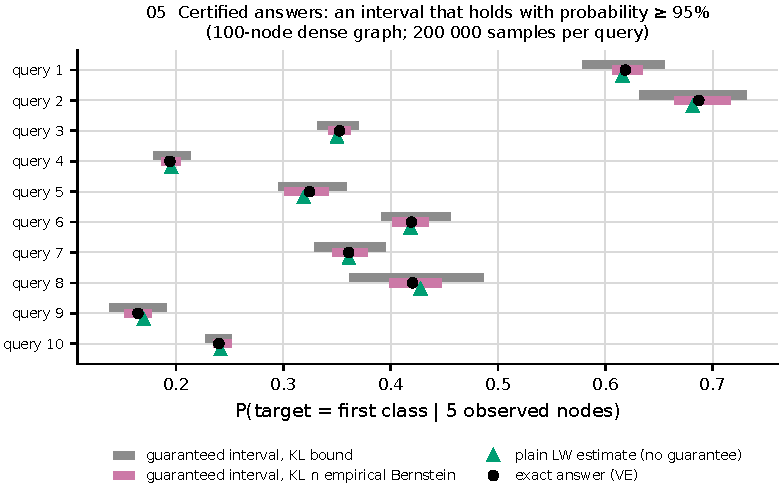
\includegraphics[width=0.72\linewidth]{05_certified_answers.pdf}
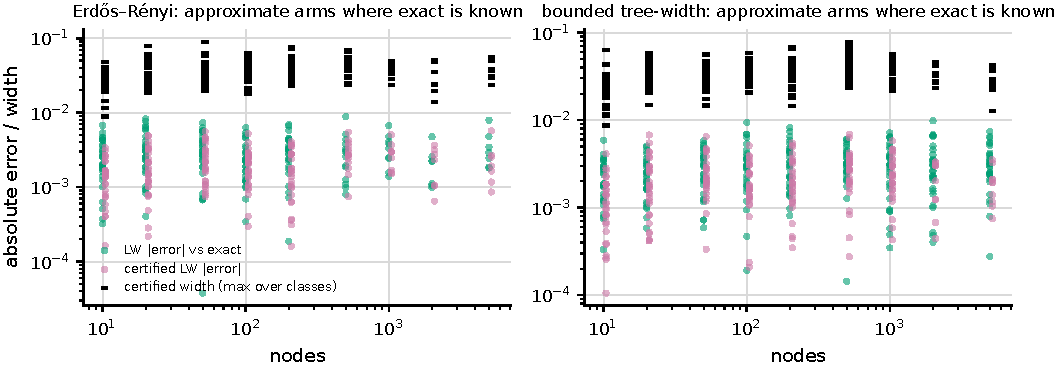
\includegraphics[width=0.9\linewidth]{discrete_approx.pdf}
\caption{Top: ten certified answers against the exact value. Bottom: errors and certified widths
for every query with an exact answer.}\label{fig:cert}
\end{figure}
\tabin{q5}
\tabin{q5t}

\subsection{S4 per-factor sets}
Per-node KL intervals take 6.3\,s for 5\,000 nodes; batched \code{interval\_sets} takes 1.0\,s,
bit-identical; closed-form L1 balls take 0.43\,s. With many parents the cost follows the table
size, and batching gains nothing (it is never slower).
\begin{figure}[H]\centering
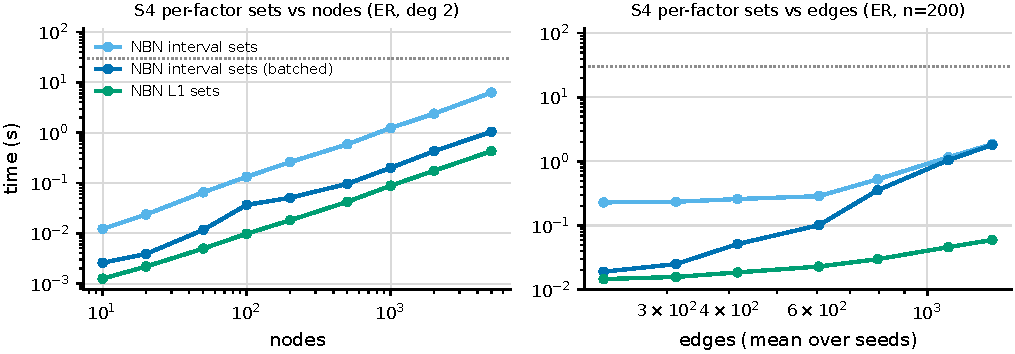
\includegraphics[width=0.85\linewidth]{discrete_sets.pdf}
\caption{S4 set builders vs nodes and edges.}\label{fig:sets}
\end{figure}

\subsection{Non-Gaussian fitting (vs Pyro)}
All three methods fit the same model for the same number of Adam steps and reach the same quality.
Stacked fitting is 3$\times$ faster than sequential NBN and 4--5$\times$ faster than Pyro at every
size, and it is flat in edges. On the GPU and on 10 threads only stacked fitting benefits; the
per-node operations of the other two are too small to parallelise.
\begin{figure}[H]\centering
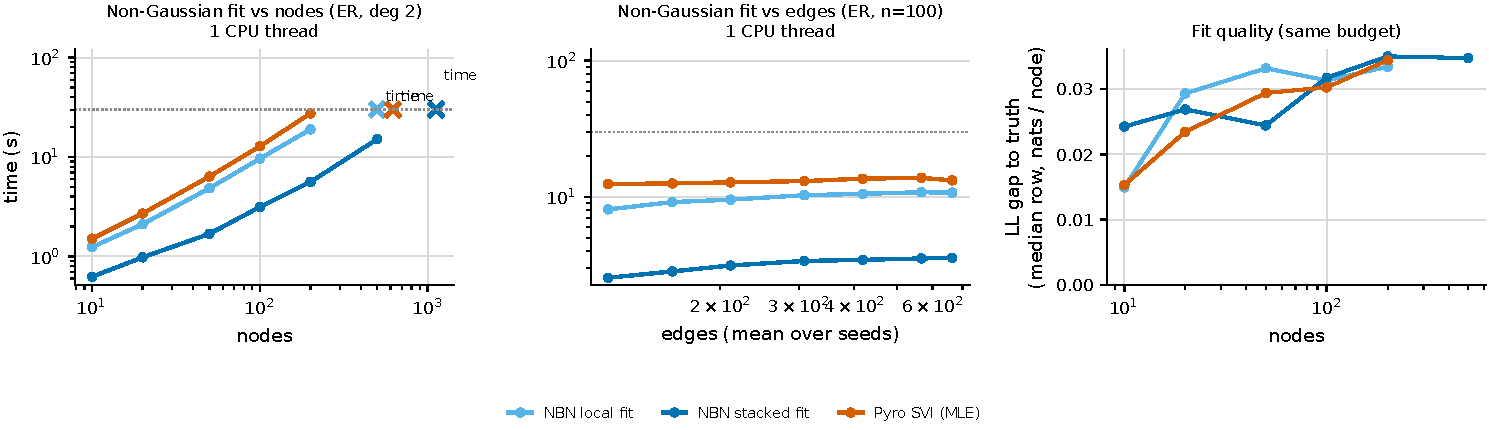
\includegraphics[width=\linewidth]{cont_fit.pdf}
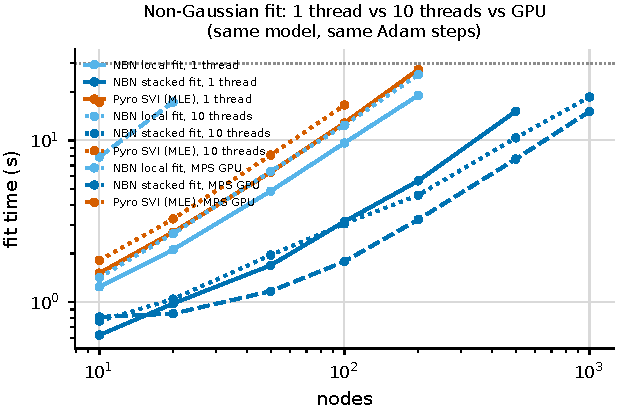
\includegraphics[width=0.62\linewidth]{cont_fit_mps.pdf}
\caption{Non-Gaussian fit: time vs nodes and edges, fit quality, and CPU vs GPU.}\label{fig:cfit}
\end{figure}

\subsection{Non-Gaussian queries (vs Pyro)}
NBN LW answers 10 queries in 0.64\,s at 2\,000 nodes and in 1.8\,s at 5\,000. NBN before takes
20.5\,s and times out; vectorised Pyro takes 23\,s and runs out of memory; \code{pyro.infer.Importance},
which draws one particle at a time, times out at 10 nodes. All three use the same estimator and
reach the same accuracy against a 4M-sample reference: median error 0.005 (NBN) and 0.004
(Pyro), 90\% quantile $\approx 0.02$. The worst error is 0.076, when the effective sample size
drops to about 0.5\%. Continuous evidence has unbounded densities, so no certified interval
exists here.
\begin{figure}[H]\centering
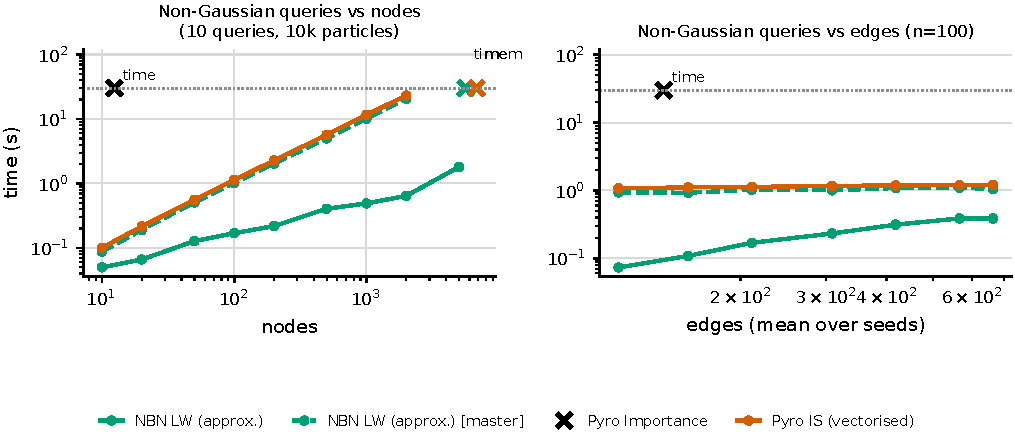
\includegraphics[width=0.85\linewidth]{cont_infer.pdf}
\caption{Non-Gaussian queries vs nodes and edges.}\label{fig:cinfer}
\end{figure}

\section{What does not scale, and why}
\begin{enumerate}
  \item \textbf{Exact inference on dense graphs}: exponential in the tree-width, and random graphs
  have tree-width growing with $n$. Pruning, evidence reduction and ordering move the wall; they
  cannot remove it.
  \item \textbf{Rare evidence}: any sampler needs $\sim 1/P(e)$ samples for relative accuracy
  (K\&F Eqs.\ 12.17--12.18, p.\ 501). \code{certified\_query} makes this visible as wide
  intervals instead of hiding it.
  \item \textbf{Many parents}: cheap to fit now, statistically poor (Fig.~\ref{fig:frag}).
  \item \textbf{Neural fitting} is linear in nodes but compute-bound: the constant was cut, the
  slope cannot be.
\end{enumerate}

\section{Verification and expert consultation}
Book experts were consulted for definitions, theorems and their conditions: \code{koller\_claude}
(Koller \& Friedman, 4 questions, including an audit of the certified construction),
\code{moss\_claude} (Algorithms for Validation, 2, including an audit),
\code{badings\_claude}, \code{causal\_abstraction\_claude} and \code{bareinboim\_claude}. Neither
audit found an error. They noted that the bounded-variable KL form of Hoeffding's bound is not in
either book (cited to the original papers instead), that the number of samples must be fixed in
advance, and suggested a sum-to-one tightening, which was applied. Four citations were checked on
primary sources.

\paragraph{Found on the way.} NBN's benchmark generator writes the mixture outputs in blocks,
\code{[locs | log-scales]}, while \code{MDNMechanism} reads them interleaved per component. So the
stock continuous non-Gaussian ground truth has scales that grow exponentially with the parents
(values up to 2\,400), against its documentation. The study uses a corrected generator; the
library generator itself is not changed.

\section{Recommendations}
\begin{enumerate}
  \item Merge the pure speed and memory changes (min-fill, induced width, LW pruning, sampling and
  passes, stacked fitting, batched sets): same answers, full test suite green.
  \item Review the new API (\code{SparseCategoricalTableMechanism}, \code{certified\_query}, width
  bounds) as a separate PR.
  \item Decide the router default (\code{query\_width\_check}): more exact answers on dense graphs,
  some of them slower.
  \item Use \code{certified\_query} as the router's fallback for discrete queries, instead of plain
  LW without a guarantee.
  \item Fix the benchmark generator's output layout; add \code{update\_local} to sparse tables;
  consider clique trees when many marginals share the same evidence.
\end{enumerate}

\appendix
\section{Reproduce}
\begin{verbatim}
cd NBN_scaling && export PYTHONPATH=$PWD
python benchmarks/scaling/run.py discrete_infer --seeds 0 1 2
python benchmarks/scaling/run.py discrete_infer_cert --seeds 0 1 2
python benchmarks/scaling/run.py discrete_fit | discrete_fit_indeg | discrete_sets
python benchmarks/scaling/run.py cont_fit [--device mps] ; ... cont_infer
python benchmarks/scaling/ref.py --particles 4000000
python benchmarks/scaling/analyze.py ; python benchmarks/scaling/explain.py
python benchmarks/scaling/report/quant_tables.py
\end{verbatim}
Raw results: \code{benchmarks/scaling/results/*.jsonl}; figures: \code{benchmarks/scaling/figures/};
full report with all tables: \code{benchmarks/scaling/README.md}.

\section{The certified query}
Run unnormalised likelihood weighting $M$ times, with $M$ fixed in advance. Particle $m$ carries
the weight $w_m=\prod_{i\in E} P(e_i\mid \mathrm{pa}_i)$ and a sampled target $Y_m$. Then
$\mathbb E[w]=P(e)$ and $\mathbb E[w\,\mathbf 1\{Y=y\}]=P(y,e)$ (K\&F Eqs.\ 12.11--12.12). Every
weight lies in $[0,W]$ with $W=\prod_i \max_{\mathrm{pa}} P(e_i\mid\mathrm{pa})$, so $w/W$ and
$w\,\mathbf 1\{Y=y\}/W$ are i.i.d.\ in $[0,1]$. For each of the $K+1$ means, take the
intersection of two intervals, each at level $\delta/(2(K+1))$:
\begin{itemize}
  \item the Chernoff--Hoeffding KL interval $\{q: M\,\mathrm{kl}(\hat\mu\|q)\leq\ln(2/\delta')\}$
  \cite{hoeffding,garivier};
  \item the empirical-Bernstein interval $\hat\mu\pm\big(\sqrt{2V\ln(2/\delta'')/M}+7\ln(2/\delta'')/(3(M-1))\big)$
  \cite{maurer}.
\end{itemize}
A union bound makes all of them hold together with probability $\geq1-\delta$. On that event,
\[ P(y\mid e)=\frac{P(y,e)}{P(e)}\in\Big[\frac{\ell_{ye}}{u_e},\ \min\Big(1,\frac{u_{ye}}{\ell_e}\Big)\Big], \]
then tightened using $\sum_y P(y\mid e)=1$. The cost grows like $W/P(e)$, the classical
relative-error regime \cite{dagum}, and does not depend on the tree-width.

\begin{thebibliography}{9}\small
\bibitem{kf} D.~Koller, N.~Friedman. \emph{Probabilistic Graphical Models}. MIT Press, 2009 (cited as K\&F, via \code{koller\_claude}).
\bibitem{hoeffding} W.~Hoeffding. Probability inequalities for sums of bounded random variables. \emph{JASA} 58(301):13--30, 1963. \url{https://doi.org/10.1080/01621459.1963.10500830}
\bibitem{garivier} A.~Garivier, O.~Cappé. The KL-UCB algorithm for bounded stochastic bandits and beyond. COLT 2011. \url{https://arxiv.org/abs/1102.2490}
\bibitem{maurer} A.~Maurer, M.~Pontil. Empirical Bernstein bounds and sample variance penalization. COLT 2009. \url{https://arxiv.org/abs/0907.3740}
\bibitem{dagum} P.~Dagum, M.~Luby. An optimal approximation algorithm for Bayesian inference. \emph{Artificial Intelligence} 93(1--2):1--27, 1997. \url{https://doi.org/10.1016/S0004-3702(97)00013-1}
\bibitem{gogate} V.~Gogate, R.~Dechter. A complete anytime algorithm for treewidth. UAI 2004, 201--208. \url{https://arxiv.org/abs/1207.4109}
\bibitem{rubenstein} P.~K.~Rubenstein et al. Causal consistency of structural equation models. UAI 2017. \url{https://arxiv.org/abs/1707.00819}
\bibitem{afv} M.~J.~Kochenderfer, S.~M.~Katz, A.~L.~Corso, R.~J.~Moss. \emph{Algorithms for Validation}. MIT Press, 2026 (via \code{moss\_claude}).
\end{thebibliography}
\end{document}
